\section{Analytical Model}

The above equation for processor utilization will hold, but $S_v$ is a
function of $v$ only through the effects of limited bandwidth. We
describe the system, model multithreading as a pipeline, derive
constraints, and discuss the limits on scheduling flexibility.

We make an initial simplification that will be relaxed later. All data
arrivals are one-to-one; that is, a task needs to suspend on one data
item that only that task is waiting on. 

\subsection{System}

For the purposes of this paper, we define a \emph{task} as a
schedulable sequence of computation. A task has its own stack, so it
can block and yield the processor when it comes to an unresolved data
dependence.

We consider a system with two levels of memory.
\begin{enumerate}
    \item \emph{Top level store}: closest memory to the processor, where
        executing task state must reside for good performance (e.g., L1 cache)
    \item \emph{Data store}: All heap data and unscheduled tasks will be
        stored here (e.g., main memory)
\end{enumerate}

We must show that the latency to the data store can be overlapped up
to the limit of bandwidth to the data store. This means that the top
level store may only contain a constant amount of state, specifically
a constant number of tasks and scheduler state.

\paragraph{Pipeline}

We will consider a dataflow multithreading system as a pipeline. The
lifecycle of a task is as follows.

Task A resides in the data store, suspended on a data dependence $D_a$.
\begin{enumerate}

    \item Task B resides in top level store and is currently executing. It
        produces $D_a$, so it marks Task A ready and copies the $D_a$ to an
        associated storage location.
    \item At some point in the future, Task A is scheduled. Its stack
        and $D_a$ start moving towards the cpu.
    \item After a time equal to the latency of the data store, the
        stack and $D_a$ arrive in the top level store. Data is
        copied to the stack, the task runs.
    \item Task A suspends on another data dependence
        Repeat 1-4 until Task A exits.

        See figure~\ref{fig:pipeline}.

\end{enumerate}

\begin{figure*}[htbp]
    \begin{center}
      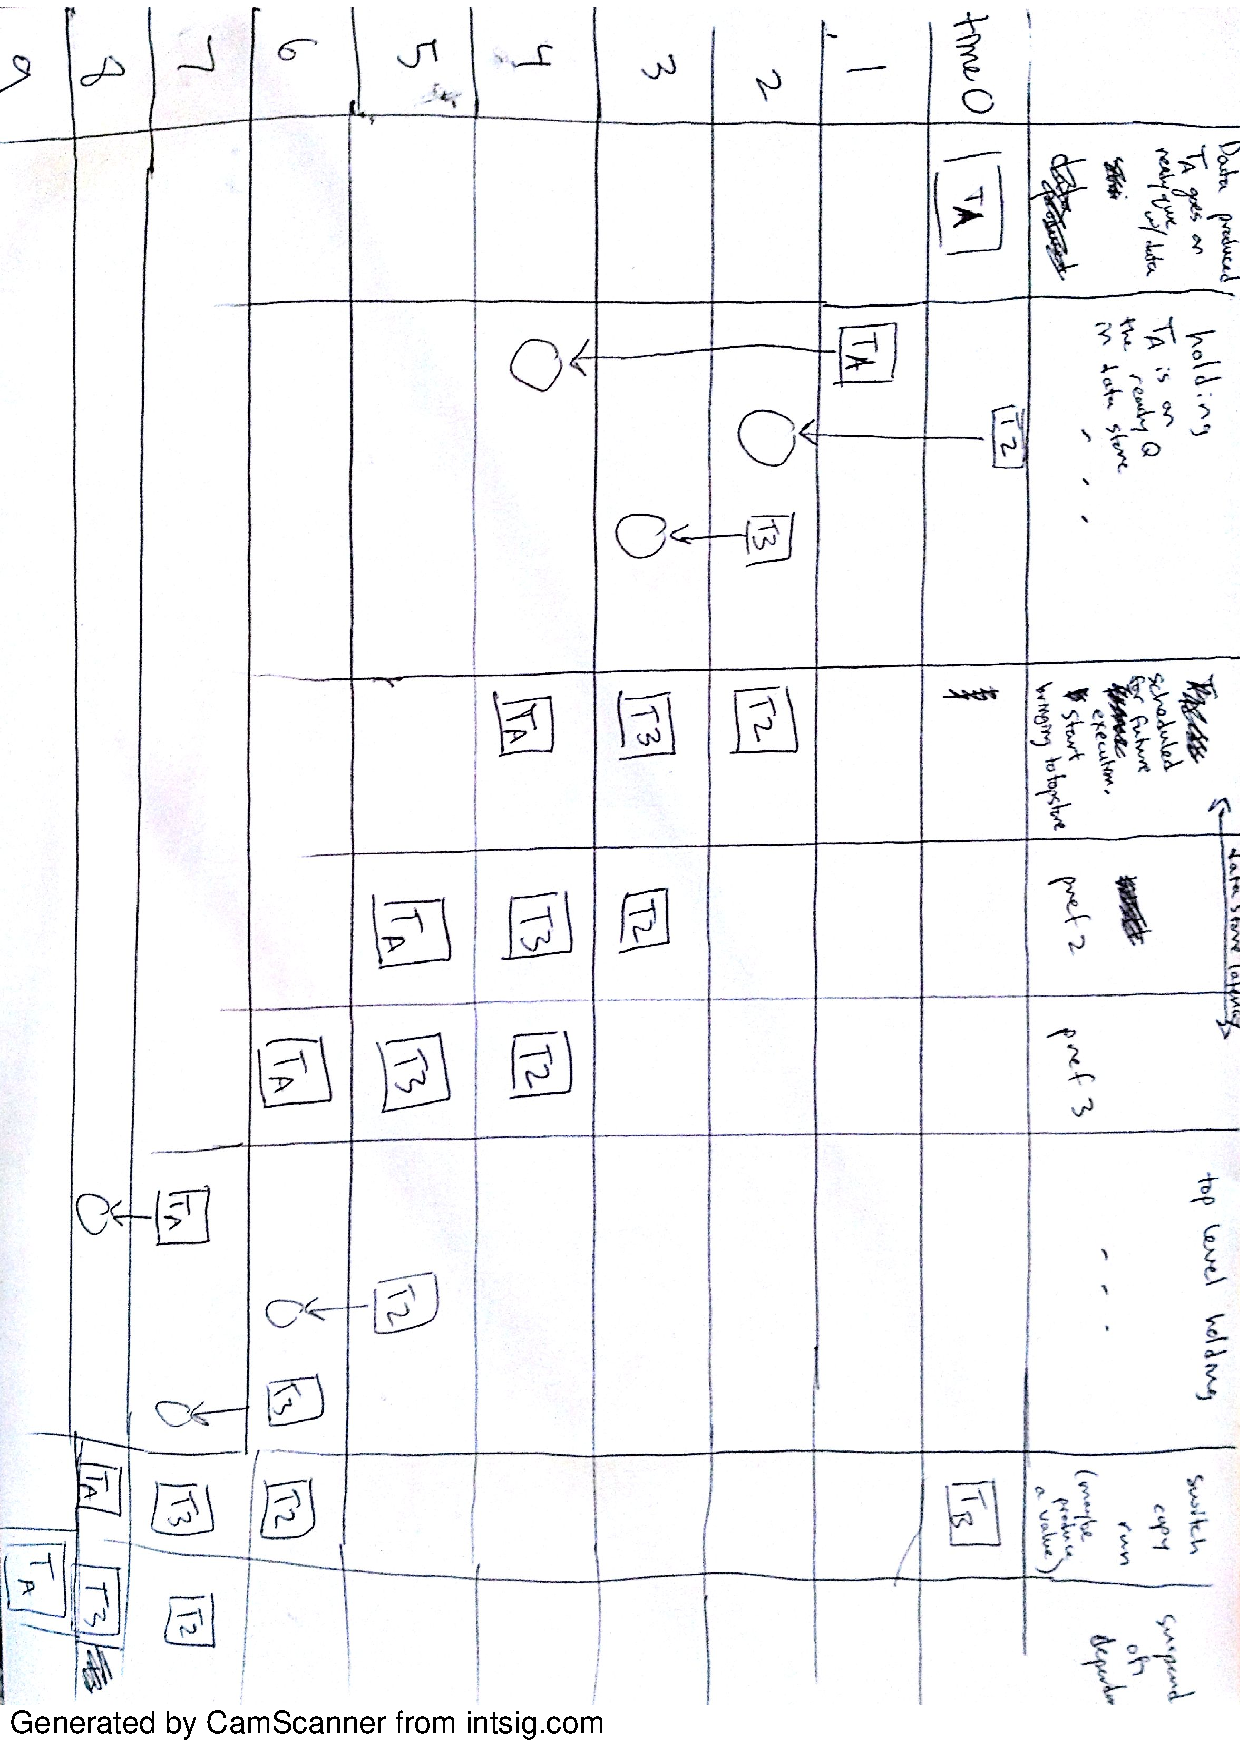
\includegraphics[width=0.7\textwidth,angle=90]{figs/pipeline.pdf}
    \end{center}
    \caption{Concpetual pipeline for dataflow multithreading}
    \label{fig:pipeline}
\end{figure*}

\paragraph{Parameters}
The parameters of the system are: 
\begin{itemize}
    \item $L_m$: latency to the data store
    \item $L_t$: latency to the top level store
    \item $B_m$: bandwidth to the data store
    \item $B_t$: bandwidth to the top level store
    \item $S_m$: size of the data store
    \item $S_t$: size of the top level store
\end{itemize}

The size of each memory level determines its latency and bandwidth
\TODO{where do we discuss bandwidth and latency, cost, physics
    relationships in depth?}

The paramters of the tasking implementation and
user program are:
\begin{itemize}
    \item $S_T$: size of a task, either some top stack frames or at most the whole stack.
    \item $T_S$: syncrhonization time between tasks
    \item $T_E$: execution time between blocking. This is assumed to
        be a single average.
    \item $S_C$: size of a \emph{candidate}, or task reference, for use by the scheduler. It
        includes at least a stack pointer but also may include
        scheduling information (e.g., a priority).
    \item $N_C$: number of candidates in the top level store.
\end{itemize}

\subsection{Constraints}
To operate in saturation mode, the processor needs a large enough
number of tasks $N_T$ to
always have useful work to overlap with memory latency. From Little's
law, $N_T \ge R_m * L_m$ \checkme{make R precise}. The size of the top
level store $S_t$ is proportional to the number of candidates and the
size of the executing task: $S_t \ge S_C * N_C + S_T$. The context
switch rate is upper bounded by the rate at which the system can read
and write tasks to the data store: $R_m \le \frac{B_m}{2*S_T}$, and is
also upper bounded by task run time and synchronization $R_m \le
\frac{1}{T_E + T_S}$.


\subsection{Relaxing one-to-one data matching}

\paragraph{Many data messages to one task}. The task
suspends once for every message that it must wait for.

\paragraph{One data message to many tasks}. When the tasks are on different
processors, there are actually multiple messages and it is the one to
one case. When the tasks are on the same processor, in stage 1 all
stack pointers can be enqueued and copies of the data.

To account for cases where a datum is produced before it is blocked
on, we can simply model a producer/consumer synchronization object as
a task (without a stack). When scheduled, the object is simply marked full. 

\TODO{some analog to tag stores in dataflow machines.
swanson's thesis has a good survey}

\section{Scheduling}

The scheduling state used to make a decision must fit in the top level
store to ensure fast context switches. This means the scheduling state
cannot grow with $N_T$, the number of required tasks. A scheduling
decision then can choose among a fixed size subset $S$ of all ready
tasks stored in the data store.

We list the places where scheduling decisions can be made and their 
implications on implementation.

\paragraph{Upon task wake}
The first place to make a scheduling decision for a task is when that
task reference is placed in the ready set. Tasks within $S$ may be
reordered. Note that the task reference must include information used for scheduling
(e.g., a priority) that is passed around by value. Once a task falls
out of $S$, it may be placed in a data structure that
does not require comparisons with other tasks on insertion (e.g., a
FIFO or a priority queue with a fixed number of priorities).
Intuitively, the ready set is a queue of references with some fixed amount of the tail in the top level
store.

\paragraph{When picking a task to prefetch}
The scheduler can pick from a subset $S$ which task to start moving
from the data store. Intuitively, the ready set is a queue of
references with some fixed amount of the head in the top level.

By scheduling at prefetch time, an implementation of pipelined
multithreading that relies on existing software prefetch instructions
cannot support arbitrary scheduling even between a fixed number of
choices. Because a future load instruction reads the task, arbitrary
scheduling would require space proportional to data store latency to
remember all the scheduling decisions in the prefetch window.

On the other hand, a context cache could support arbitrary scheduling
decisions over a fixed window of tasks. \TODO{do we want to expand on
    this}

\paragraph{When picking a task to run}


\subsection{Implementation}
If scheduling at prefetch time, general software prefetch and load instructions in modern processors
cannot provide the required functionality for arbitrary constant size
scheduling. Because the address must be prefetched and later loaded,
the scheduler would need to keep track of the scheduling decisions
made on prefetch to load in the same order. 
